%==============================================================================
% CHAPITRE 3 : RÉALISATION
%==============================================================================
\chapter{Réalisation}

\section{Environnement de développement}

\subsection{Stack technologique}

Le tableau~\ref{tab:technologies} récapitule l'ensemble des technologies utilisées pour la réalisation du projet.

\begin{table}[H]
\centering
\renewcommand{\arraystretch}{1.4} % Aère les lignes sans surcharger la hauteur du tableau
\caption{Stack technologique du projet SmartBI}
\label{tab:technologies}
\begin{tabularx}{\textwidth}{
    >{\raggedright\arraybackslash\bfseries}l 
    >{\raggedright\arraybackslash}l 
    >{\raggedright\arraybackslash}X
}
\toprule
\textbf{Catégorie} & \textbf{Technologie} & \textbf{Rôle} \\
\midrule
Framework backend  & Django 6.0                 & Framework web Python avec DRF pour l'API REST \\
CORS               & django-cors-headers       & Gestion des requêtes cross-origin \\
Orchestration IA   & LangGraph                  & Framework de graphes d'état pour agents multi-agents \\
LLM local          & Ollama                     & Serveur d'inférence pour modèles de langage locaux \\
Modèle LLM         & Qwen3-Coder                & Modèle de langage utilisé pour l'inférence \\
Prompts            & LangChain (core + ollama)  & Templates de prompts et connecteur LLM \\
Analyse données    & Pandas + openpyxl          & Lecture et transformation de fichiers CSV/XLSX \\
Base de données    & SQLite                     & Stockage léger embarqué pour les données BI \\
Framework frontend & React 19                   & Bibliothèque UI pour l'interface monopage \\
Build tool         & Vite 8                     & Bundler et serveur de développement rapide \\
Routing            & react-router-dom 7         & Routage SPA côté client \\
Visualisation      & Recharts 3.8               & Graphiques interactifs basés sur D3.js \\
IDE                & VS Code                    & Éditeur de code principal \\
Versioning         & Git                        & Suivi des modifications du code source \\
\bottomrule
\end{tabularx}
\end{table}

\subsection{Organisation du projet}

Le projet est organisé en deux modules principaux : le module frontend (\texttt{frontend\_bi/}) contenant l'application React avec ses pages, composants et contexte global, et le module backend (\texttt{pfa\_backend/}) contenant le projet Django avec l'application \texttt{api\_bi} qui héberge le pipeline d'agents, le module d'ingestion et les vues API. Les deux modules communiquent exclusivement via l'API REST.

\section{Réalisation du backend}

\subsection{Configuration et points d'API}

Le backend Django est configuré avec le middleware CORS en tête de chaîne pour autoriser les requêtes depuis le frontend React. Deux endpoints REST sont exposés, présentés dans le tableau~\ref{tab:endpoints}.

\begin{table}[H]
\centering
\renewcommand{\arraystretch}{1.5} % Aère le tableau pour une meilleure lisibilité
\caption{Endpoints de l'API REST SmartBI}
\label{tab:endpoints}
\begin{tabularx}{\textwidth}{
    >{\raggedright\arraybackslash\bfseries}l 
    >{\centering\arraybackslash}p{2cm} 
    >{\raggedright\arraybackslash}X
}
\toprule
\textbf{Endpoint} & \textbf{Méthode} & \textbf{Description} \\
\midrule
/api/upload/   & POST & Ingestion de fichier CSV/XLSX et proposition de nettoyage des colonnes (NDJSON) \\
/api/confirm\_upload/ & POST & Validation du nettoyage, écriture en base et exécution du pipeline d'agents (NDJSON) \\
/api/generate/ & POST & Génération d'un dashboard à partir d'une question en langage naturel \\
\bottomrule
\end{tabularx}
\end{table}

\subsection{Upload avec streaming de progression et nettoyage}

L'upload de fichiers exploite le mécanisme de \texttt{StreamingHttpResponse} de Django pour envoyer des mises à jour de progression en temps réel au format NDJSON (Newline Delimited JSON). L'ingestion se déroule en deux phases : d'abord le téléversement (\texttt{/api/upload/}) où l'Agent Column Cleaner propose des colonnes à supprimer, puis après validation par l'utilisateur (\texttt{/api/confirm\_upload/}), l'écriture en base et l'analyse.

Le frontend lit cette réponse flux par flux via l'API \texttt{ReadableStream} du navigateur, affichant une barre de progression animée avec le nom de l'agent en cours d'exécution. Les étapes de progression incluent : ingestion (10\%), nettoyage des colonnes (25\%), attente de validation (30\%), application des suppressions (35\%), explication par l'IA (40\%), analyse par l'agent analyste (55\%), requêtage par l'agent ingénieur (70\%), conception du dashboard par l'agent designer (85\%), et finalisation (100\%).

\subsection{Pipeline multi-agents LangGraph}

Le pipeline est implémenté comme un graphe d'état LangGraph compilé une seule fois au chargement du module et réutilisé pour chaque requête. Il orchestre trois agents spécialisés : l'analyste qui propose les KPIs, l'ingénieur qui génère et exécute les requêtes SQL, et le designer qui produit le JSON du dashboard. Un mécanisme de retry avec feedback d'erreur permet jusqu'à trois tentatives en cas d'échec SQL.

Cinq templates de prompts distincts, tous rédigés en français, guident les agents dans leurs rôles respectifs : analyste conversationnel, analyste automatique, ingénieur SQL, designer de dashboard et explainer de dataset.

\section{Réalisation du frontend}

\subsection{Architecture de l'application}

L'application React est structurée selon une architecture par pages avec un composant racine définissant le layout global et les routes. Le contexte global (\texttt{BiPlatformContext}) encapsule un \texttt{useReducer} avec persistance dans le navigateur, assurant la continuité entre les sessions.

\subsection{Page de chargement de données}

La page d'accueil offre une zone de glisser-déposer interactive pour les fichiers CSV et XLSX. Après soumission, une barre de progression gradient indique l'avancement du pipeline avec le nom de l'agent actif. À la fin du traitement, l'utilisateur est redirigé automatiquement vers le tableau de bord global.

\begin{figure}[H]
\centering
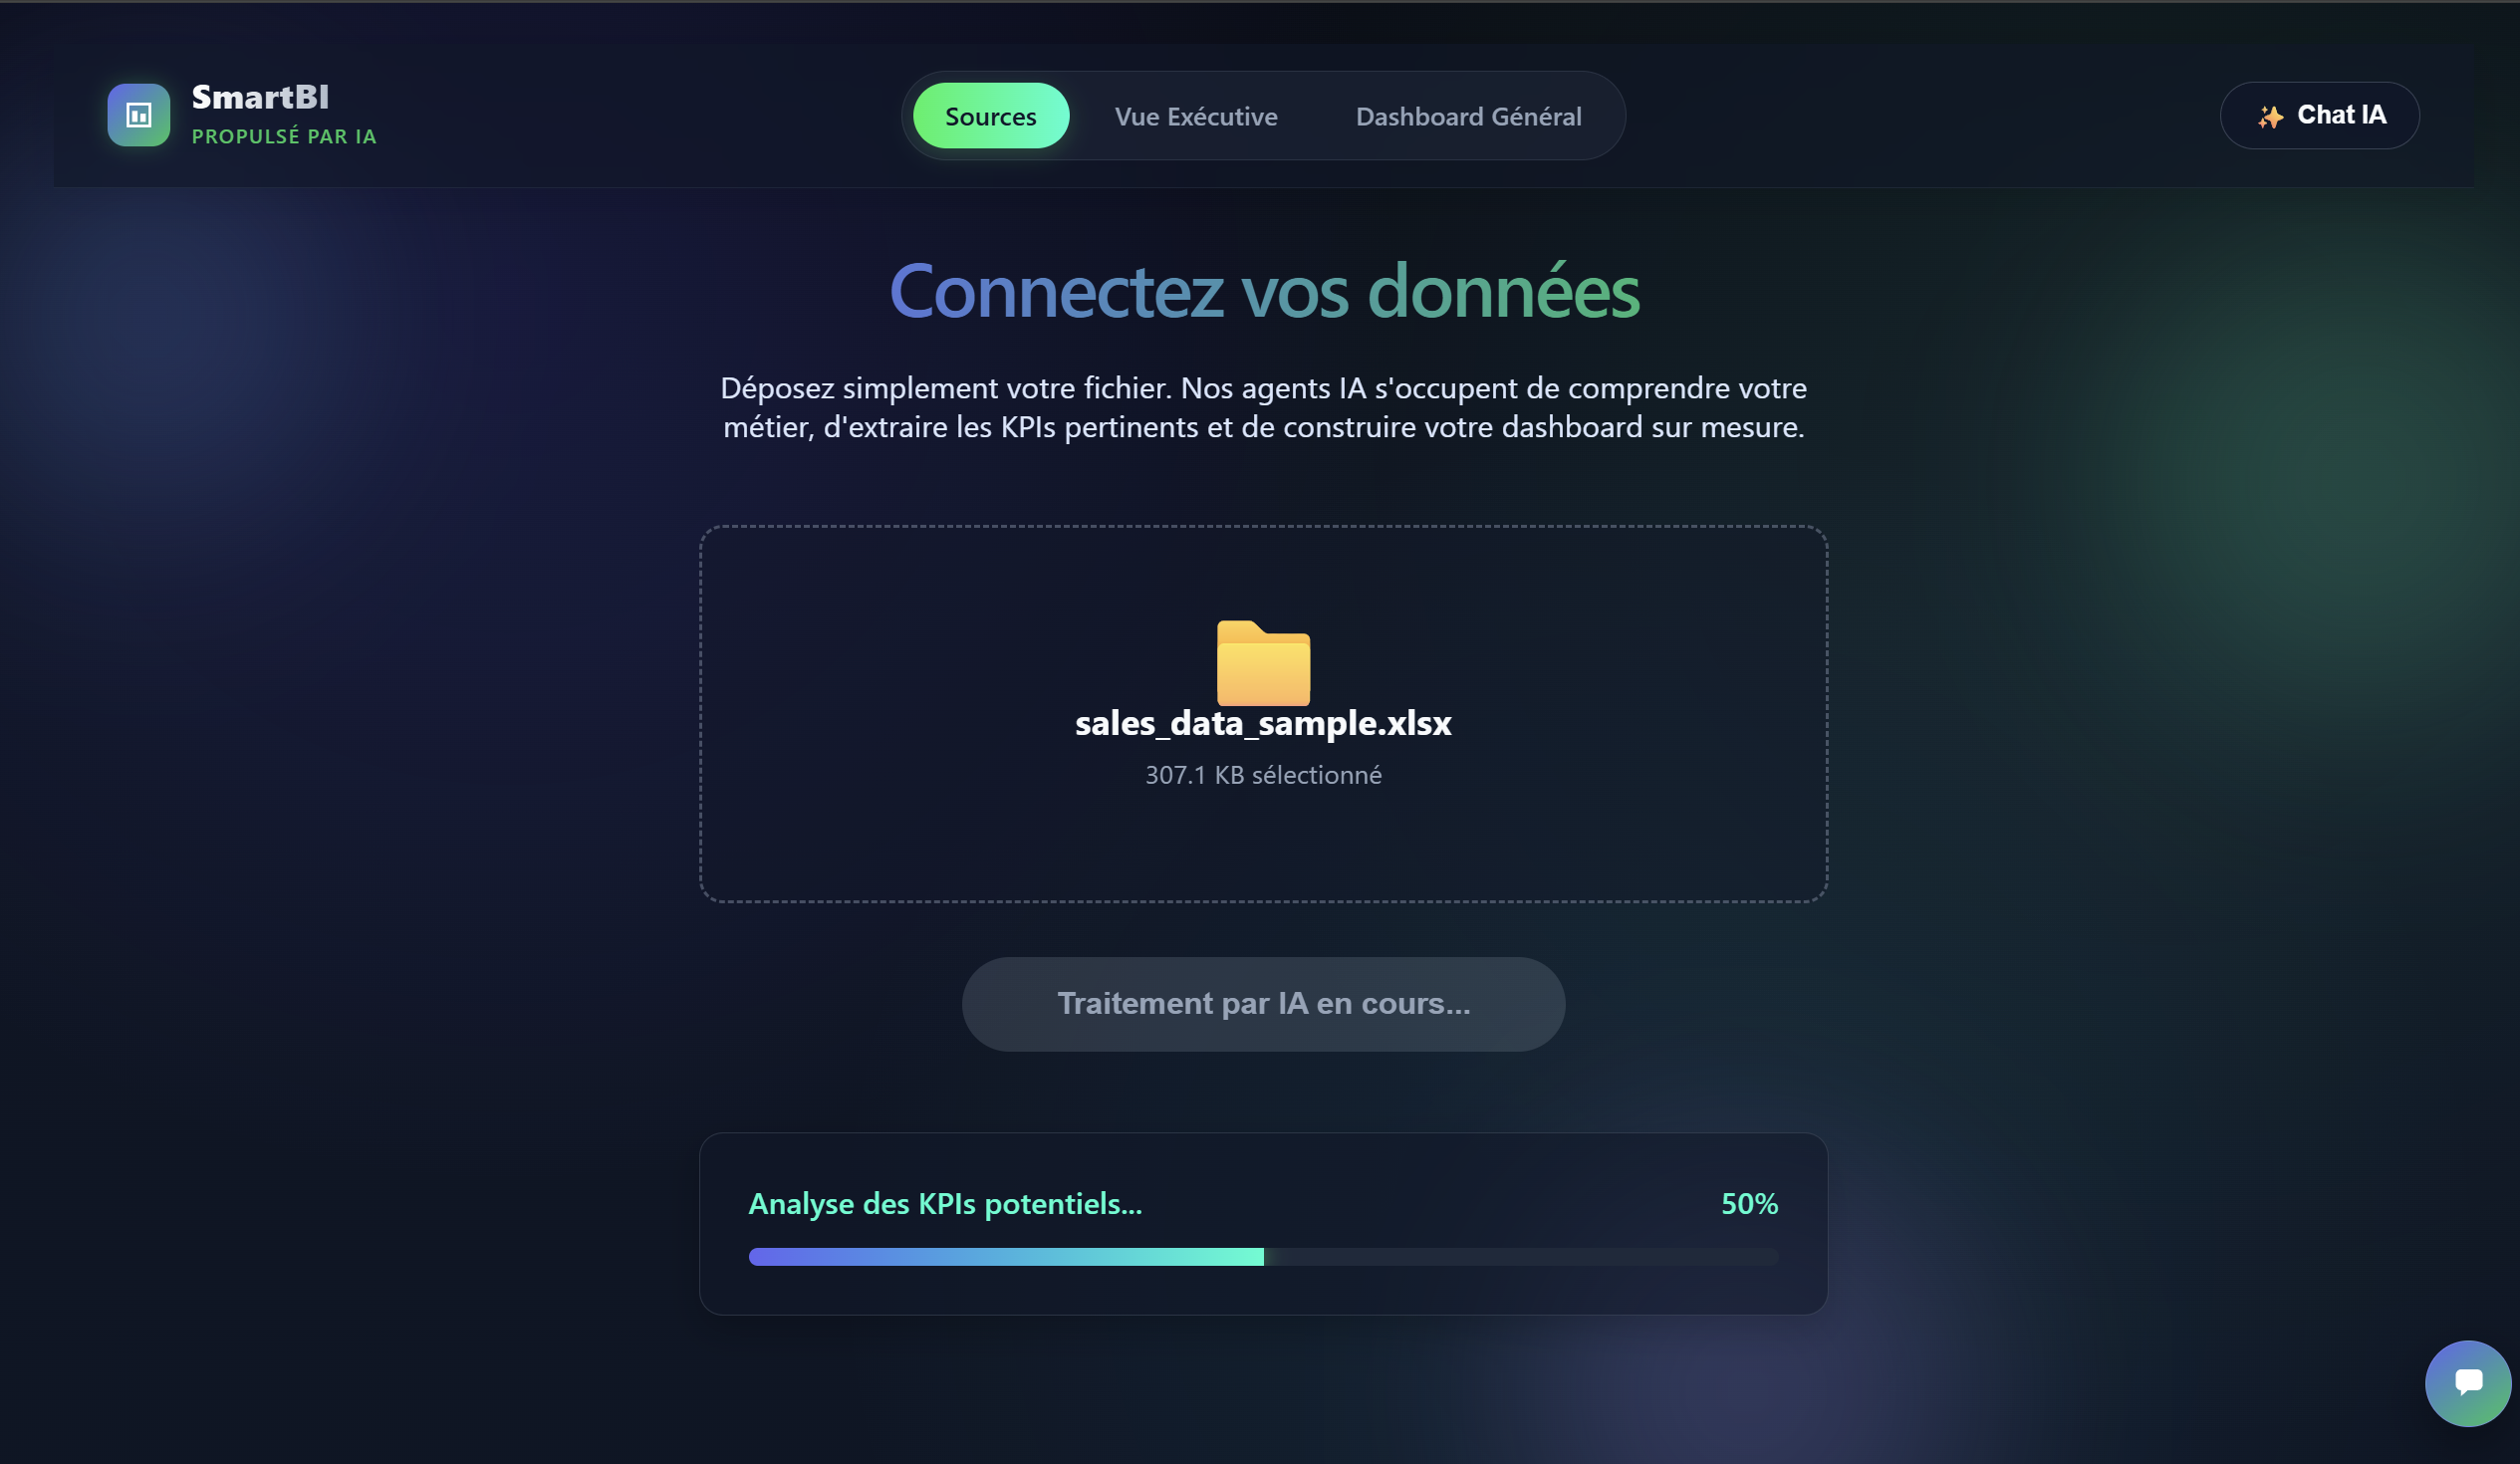
\includegraphics[width=\textwidth]{Smartbi/Screenshot 2026-06-22 173804.png}
\caption{Progression du pipeline d'agents lors de l'upload}
\label{fig:progress}
\end{figure}

\subsection{Tableau de bord global}

Le tableau de bord global présente un résumé exécutif de la santé des données sous forme de six cartes métriques : nombre de lignes, nombre de colonnes, taux de complétude moyen, colonnes numériques, colonnes à risque (nullité $\geq 20\%$) et pourcentage moyen de valeurs nulles. Un panneau d'explication contextuelle générée par l'IA accompagne ces indicateurs, suivi d'un tableau détaillé de chaque colonne avec ses statistiques descriptives.


\begin{figure}[H]
\centering
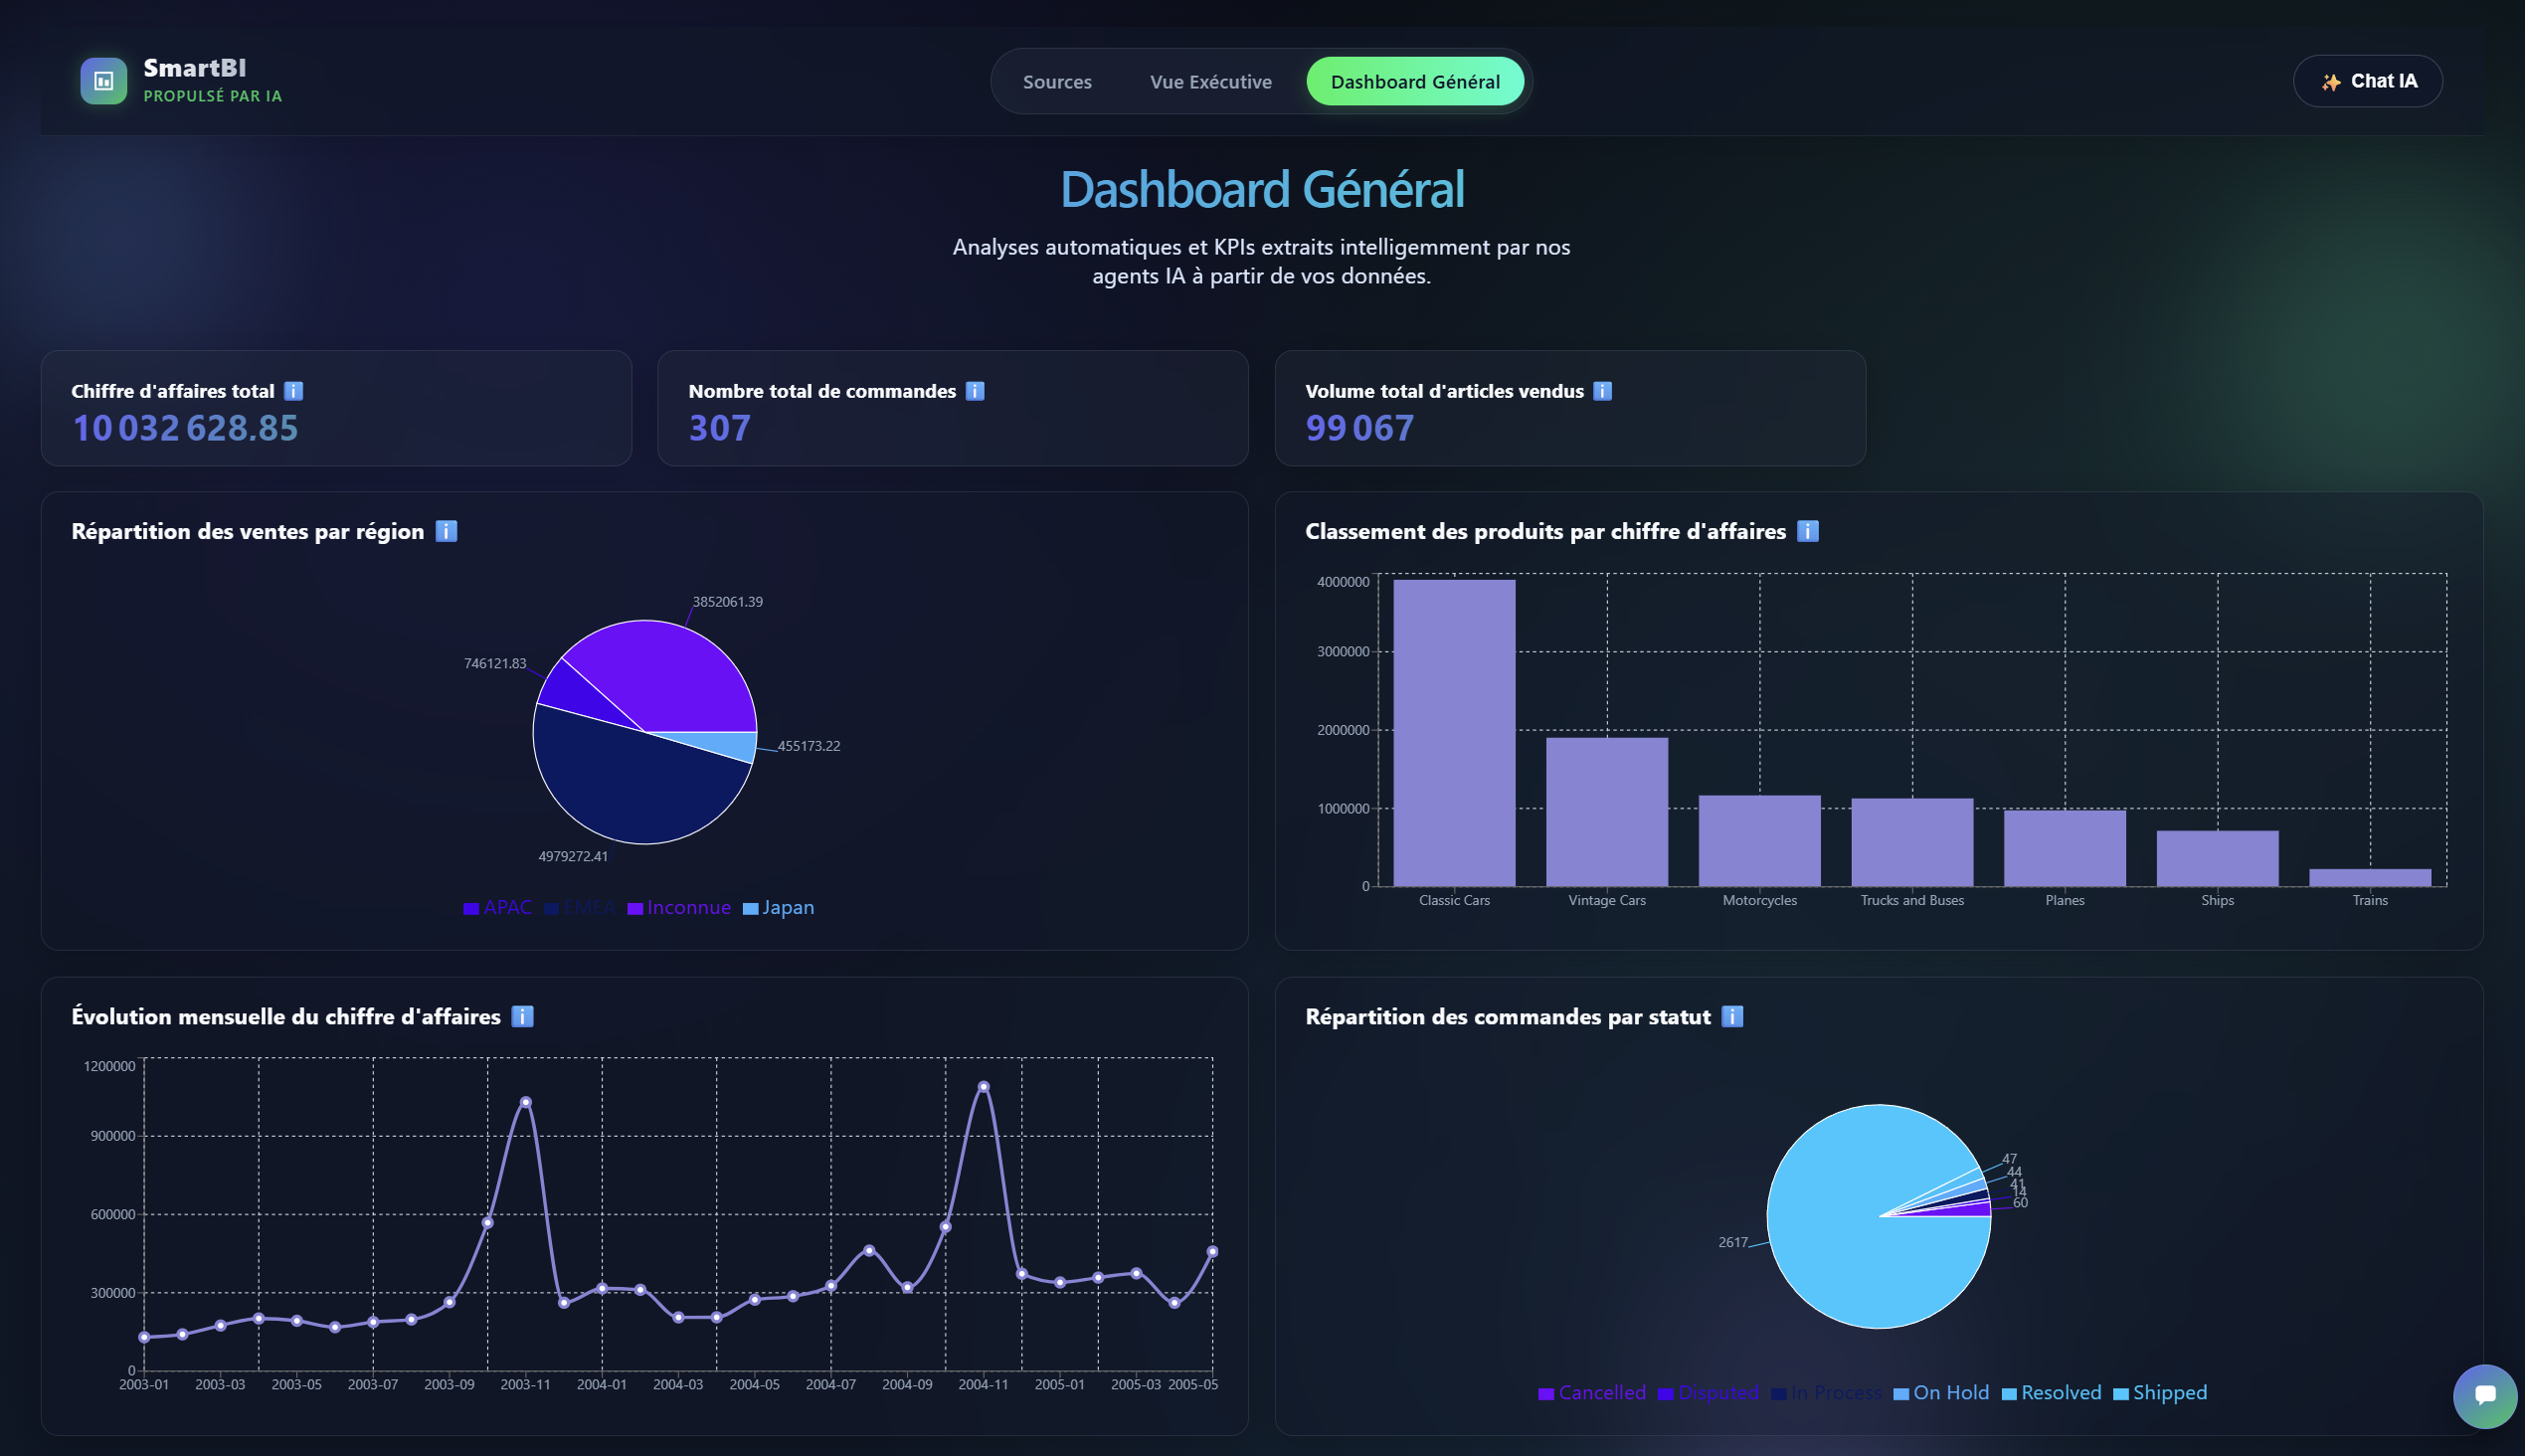
\includegraphics[width=\textwidth]{Smartbi/Screenshot 2026-06-22 181010.png}
\caption{Filtrage temporel dynamique des indicateurs}
\label{fig:filtrage}
\end{figure}

\subsection{Page des insights avec filtrage temporel}

La page des insights rend le tableau de bord généré automatiquement par le pipeline d'agents. Elle implémente un système de filtrage par période qui calcule les options appropriées selon les plages de dates détectées dans les données (jours, mois, années). Les widgets sont disposés dans une grille responsive combinant MetricCards, BarCharts, PieCharts et LineCharts.



\begin{figure}[H]
\centering
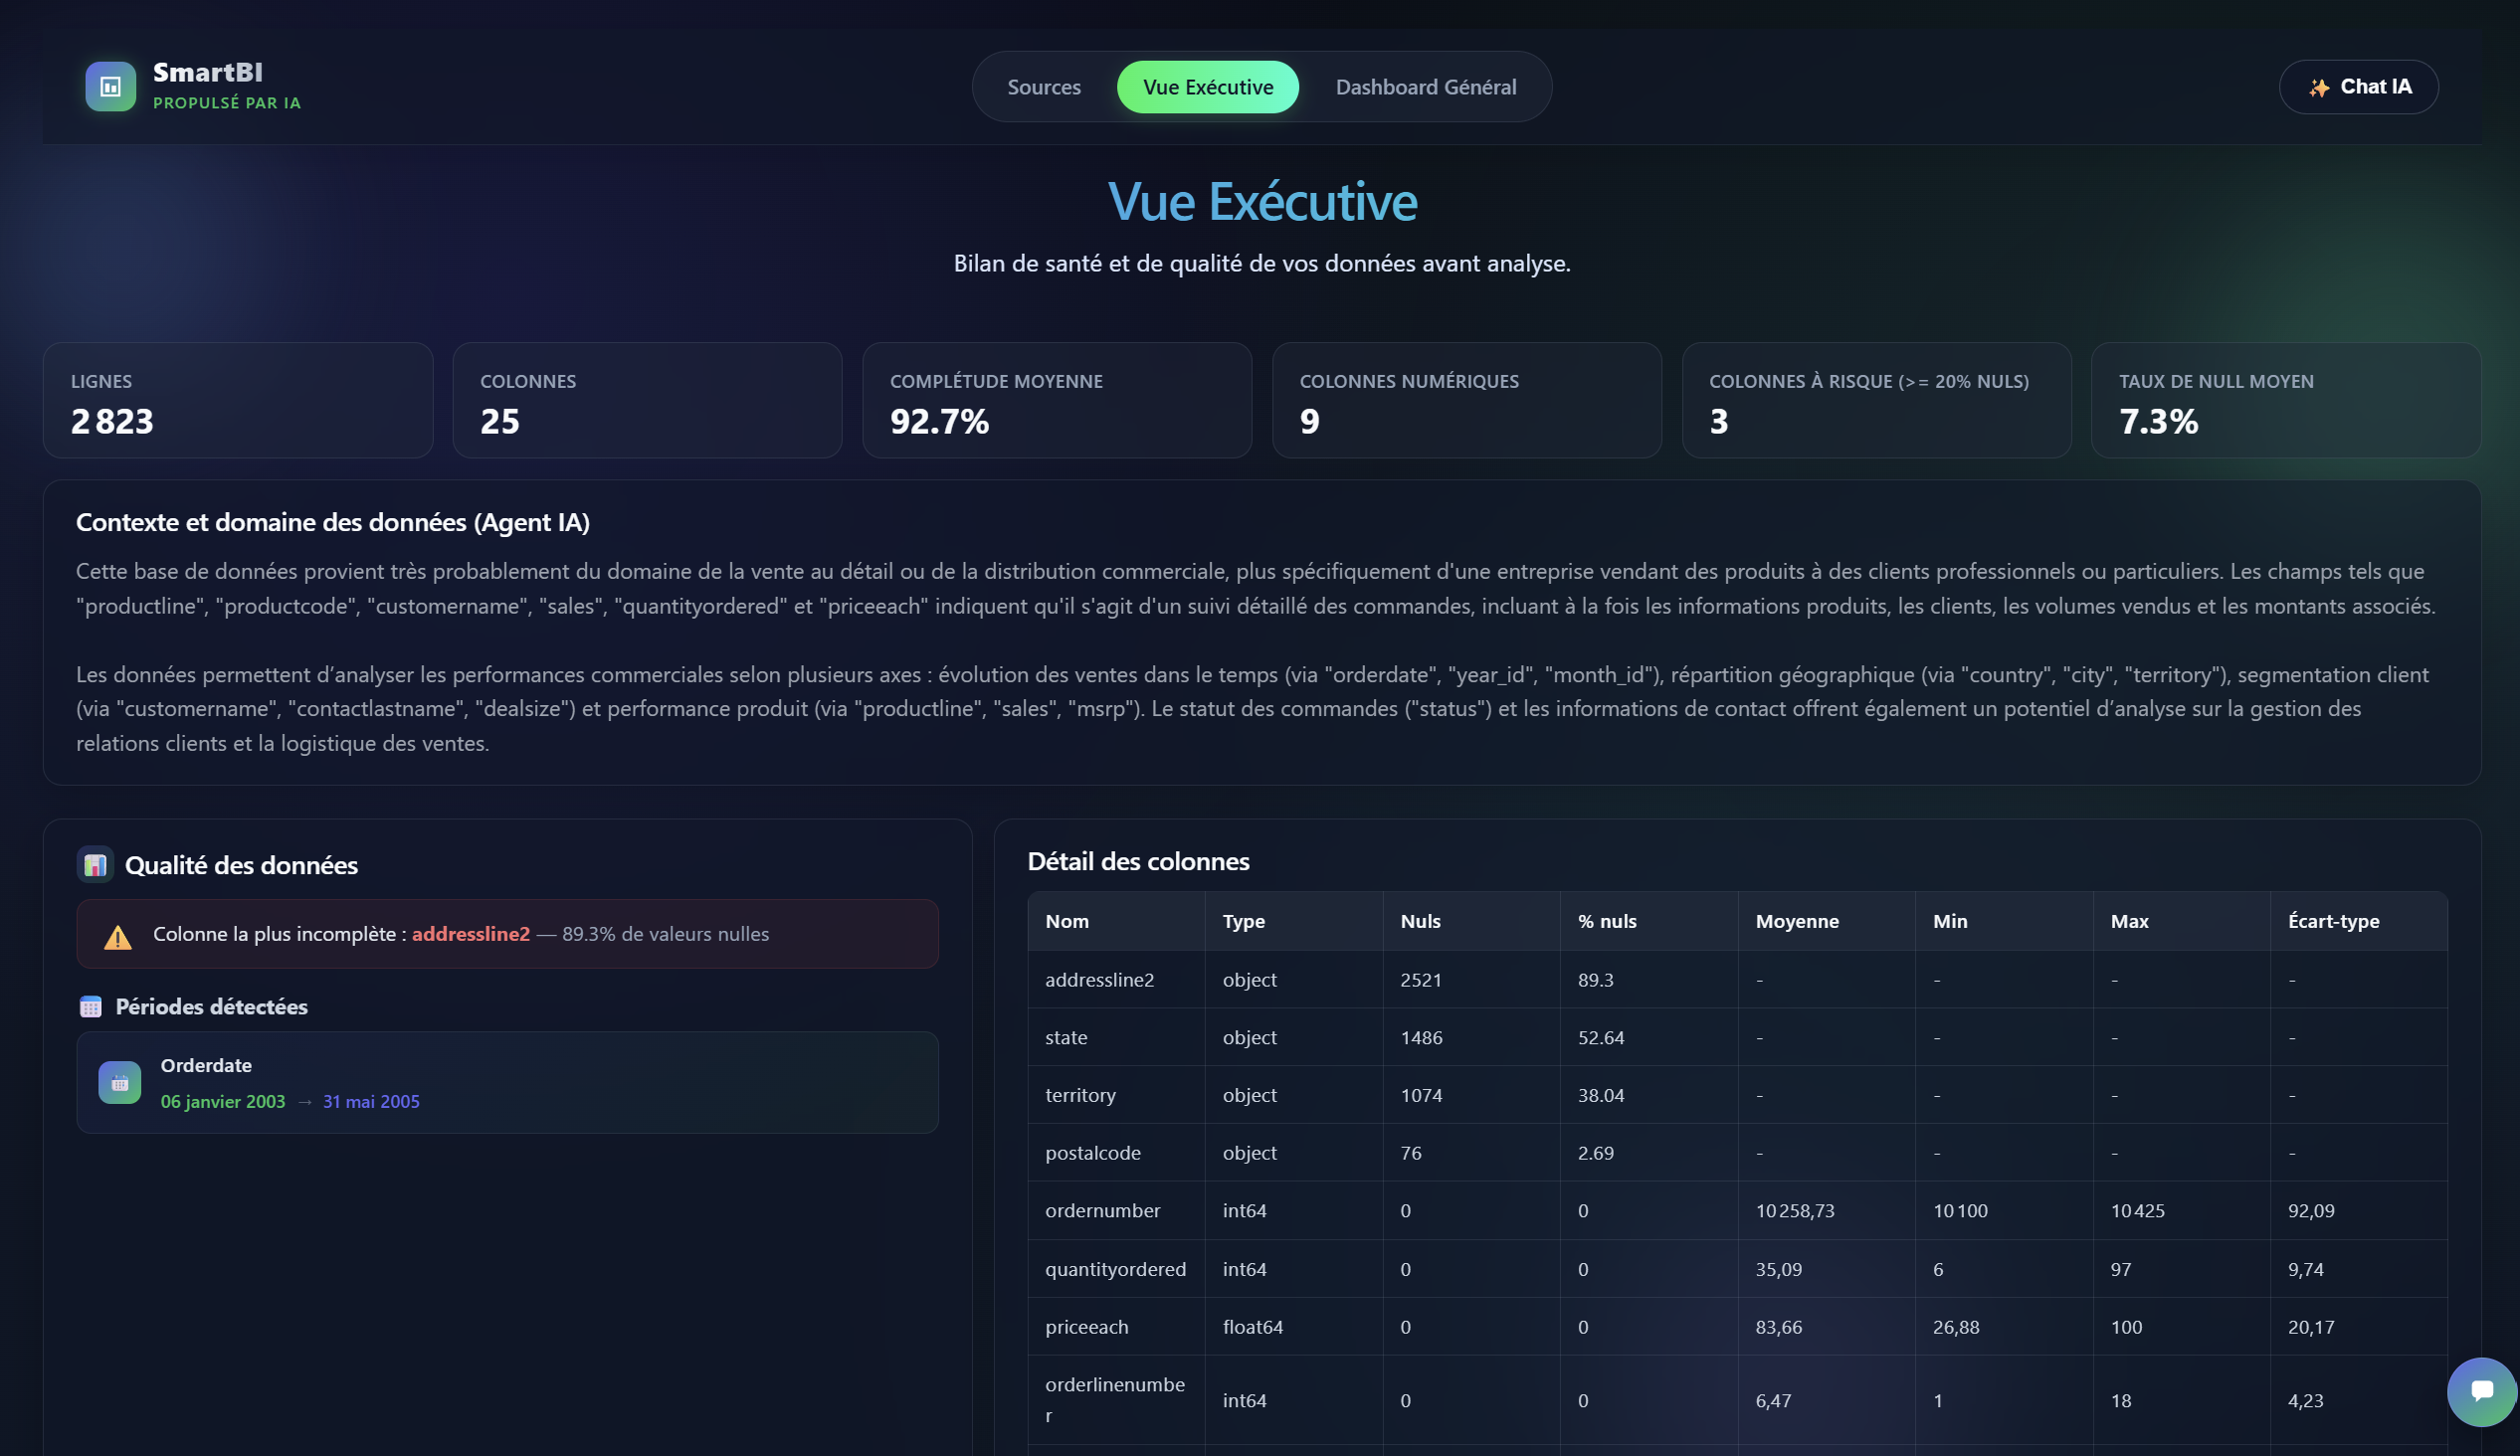
\includegraphics[width=\textwidth]{Smartbi/Screenshot 2026-06-22 180721.png}
\caption{Page des insights --- tableau de bord généré par les agents IA}
\label{fig:filtrage}
\end{figure}

\subsection{Interface de conversation IA}

L'interface de chat offre une expérience conversationnelle fluide avec des bulles de message stylisées et une barre de saisie fixe en bas de page. Afin d'améliorer l'expérience utilisateur et de simuler le temps de réflexion de l'IA, une animation de chargement (trois petits points formant une vague) s'affiche de manière dynamique pendant l'attente de la réponse. Les visualisations générées par l'IA s'affichent ensuite directement dans le fil de conversation, en dessous du message textuel de l'agent. L'assistant est également accessible via un panneau latéral activé par un bouton flottant.



\begin{figure}[H]
\centering
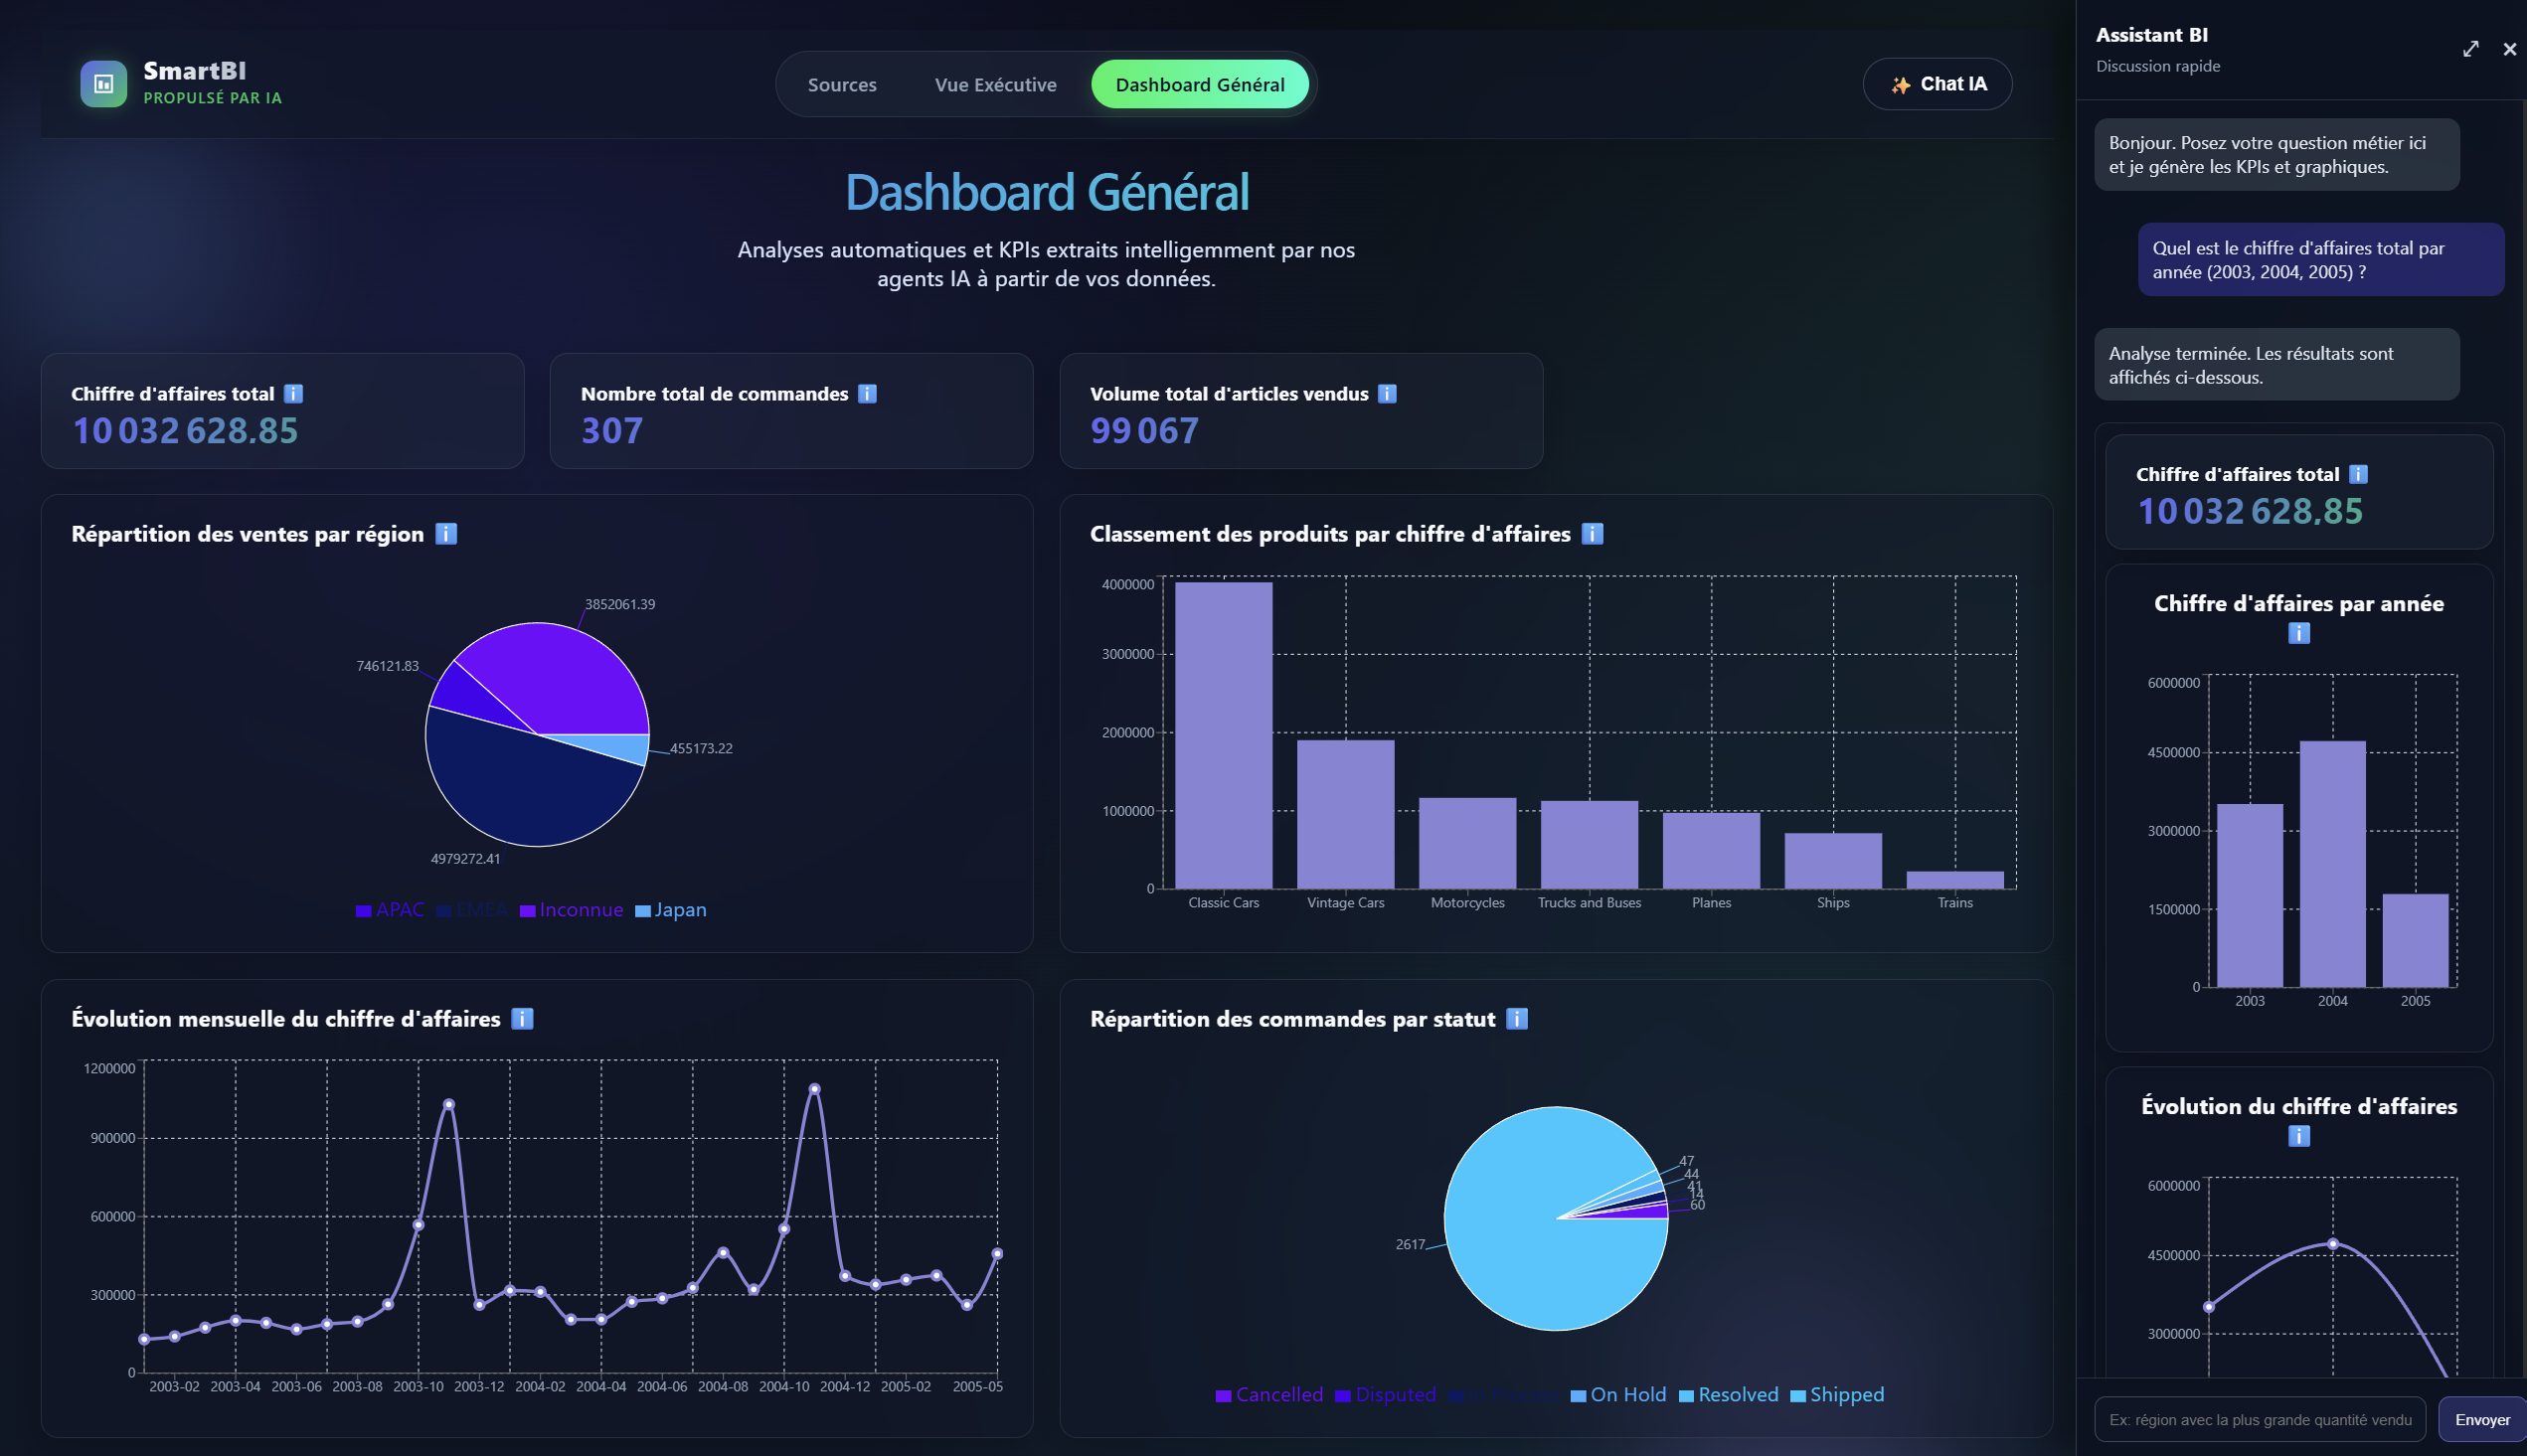
\includegraphics[width=\textwidth]{Smartbi/Screenshot 2026-06-22 181201.png}
\caption{Panneau latéral de conversation IA}
\label{fig:chat-panel}
\end{figure}

\section{Scénarios d'utilisation}

\subsection{Scénario 1 : Analyse automatique d'un fichier de ventes}

Un utilisateur charge un fichier CSV contenant des données de ventes (date, produit, région, quantité, prix unitaire, montant total). Le système ingère les données, génère une explication contextuelle, propose 8 KPIs (chiffre d'affaires total, panier moyen, ventes par région, évolution mensuelle, top 5 produits, etc.), exécute les requêtes SQL et produit un dashboard complet combinant cartes métriques et graphiques variés.


\begin{figure}[H]
\centering
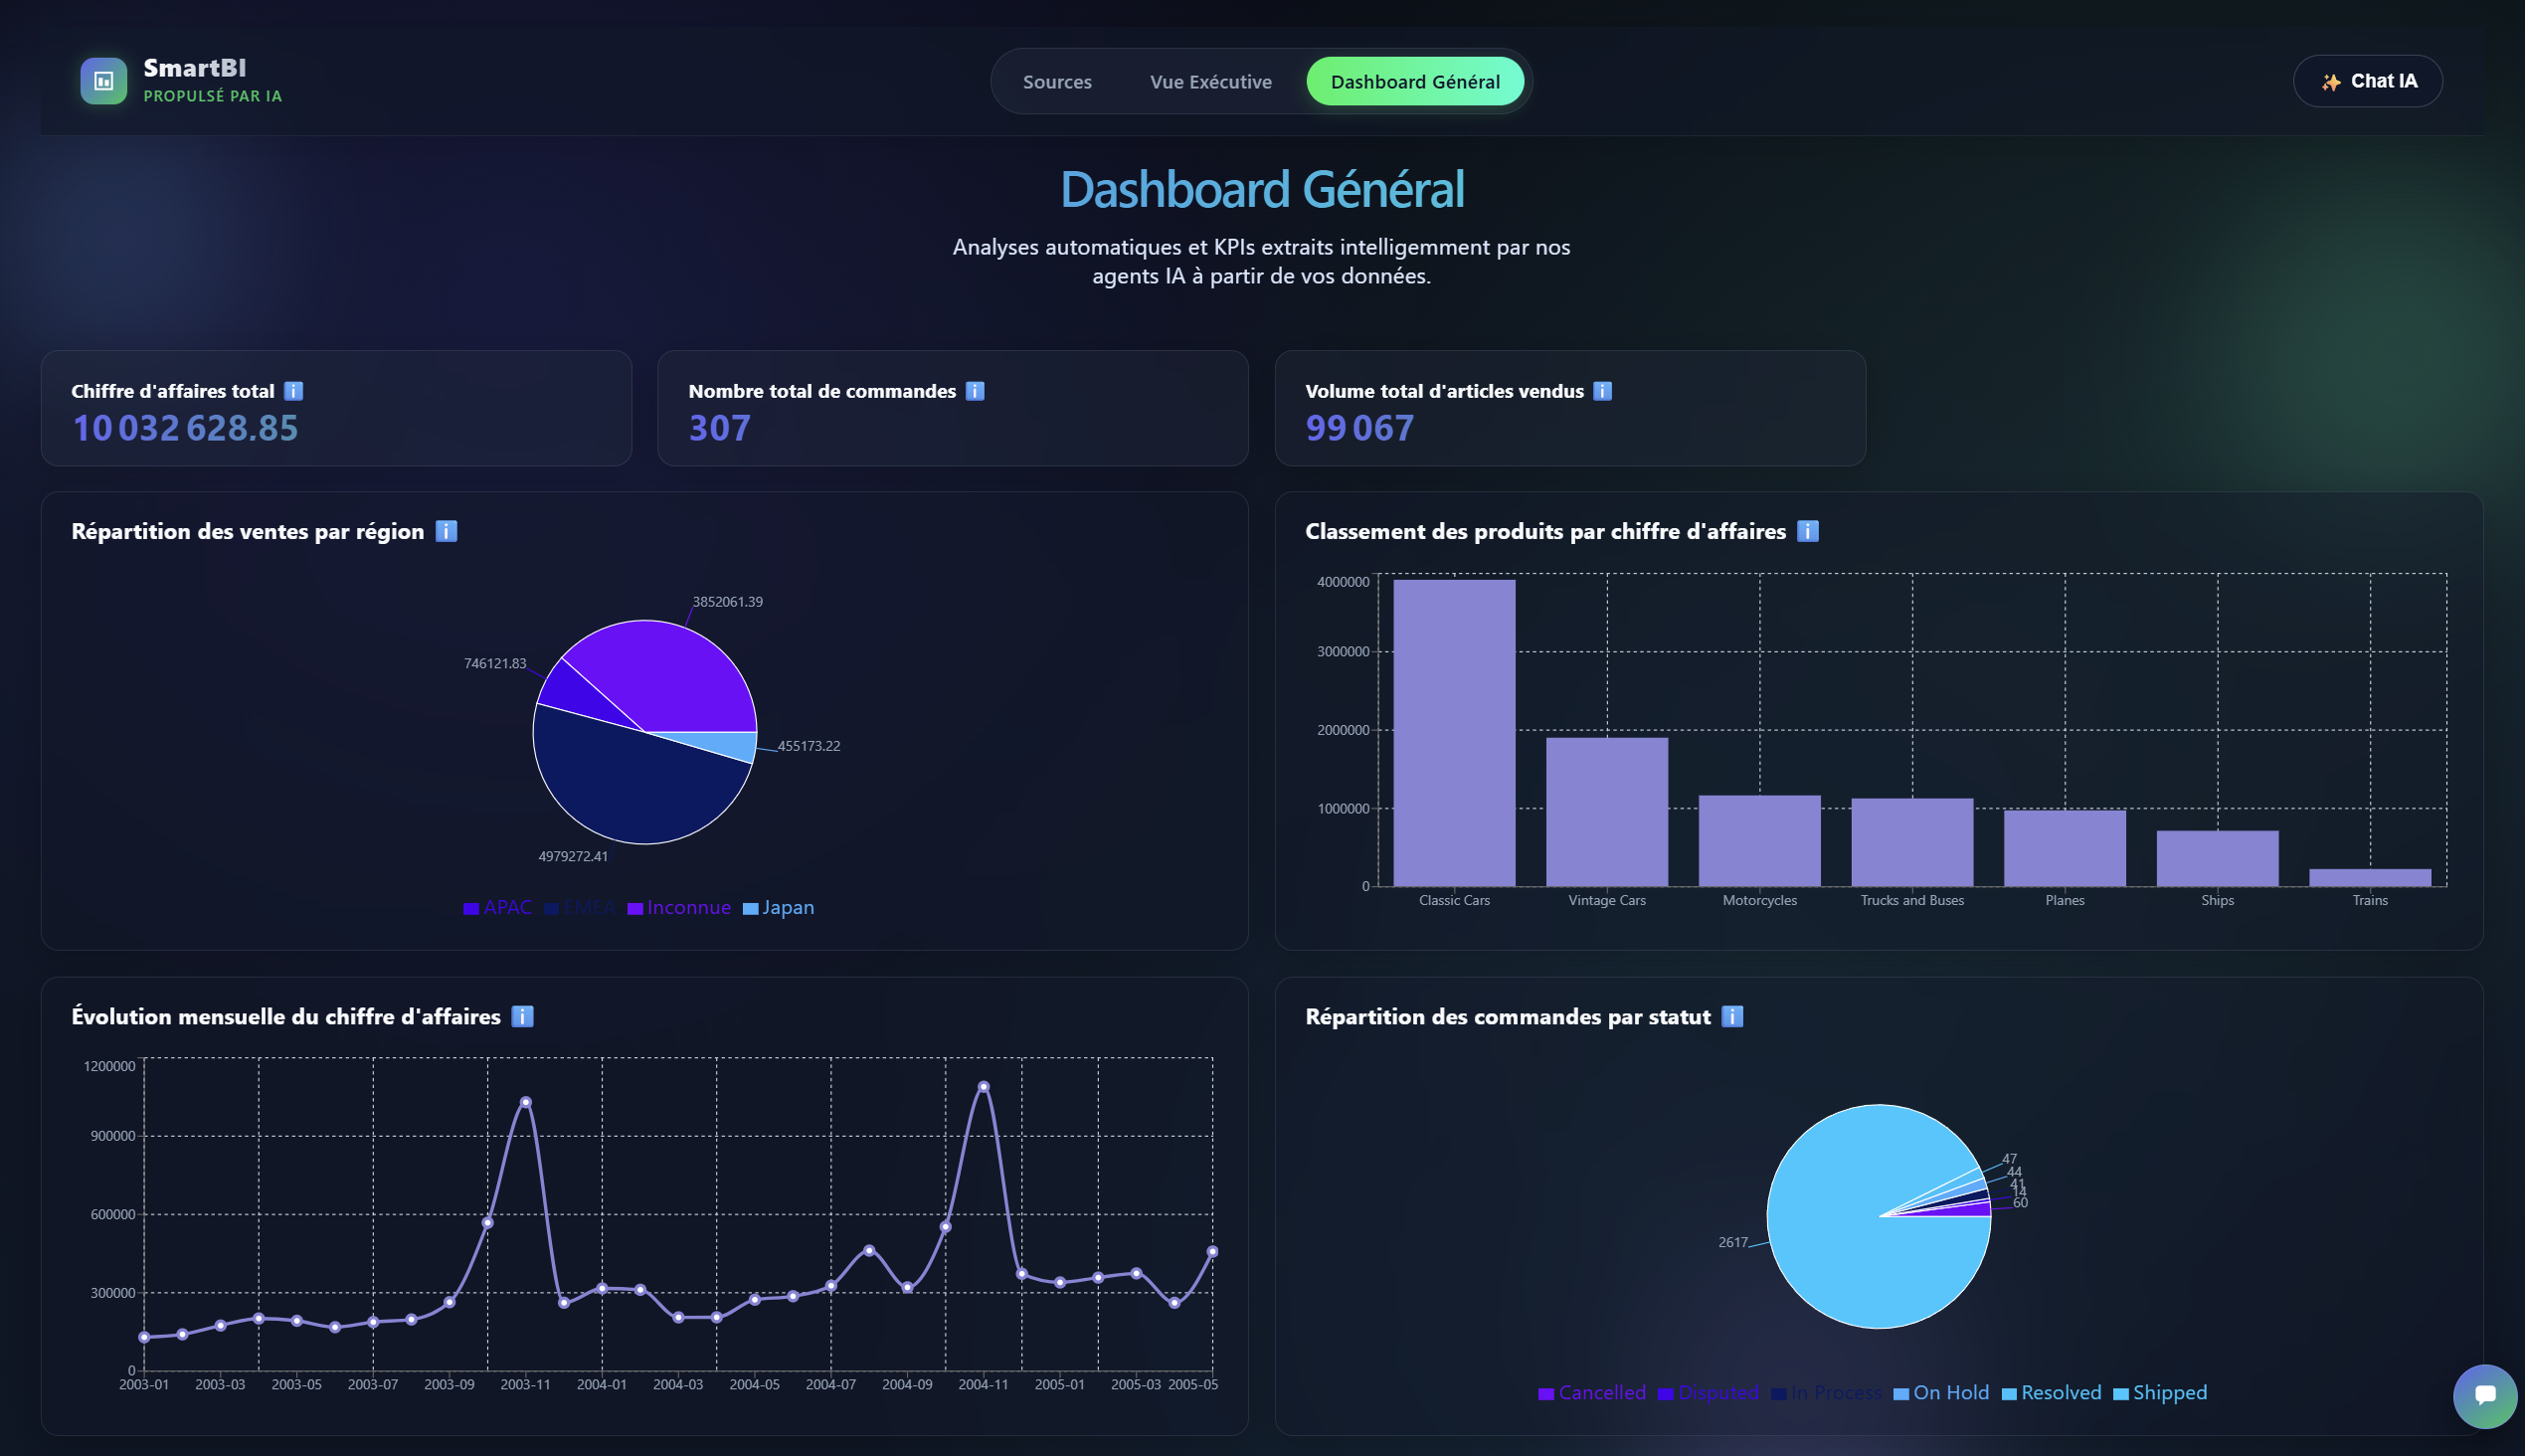
\includegraphics[width=\textwidth]{Smartbi/Screenshot 2026-06-22 181010.png}
\caption{Dashboard généré automatiquement à partir du fichier de ventes}
\label{fig:filtrage}
\end{figure}


\subsection{Scénario 2 : Question conversationnelle}

Après avoir chargé ses données, l'utilisateur pose la question : «~Quel est le produit le plus vendu par mois~?~» Le système active le mode conversationnel, l'analyste identifie le KPI pertinent, l'ingénieur génère la requête SQL avec agrégation mensuelle, et le designer produit un graphique affiché inline dans la conversation.



\begin{figure}[H]
\centering
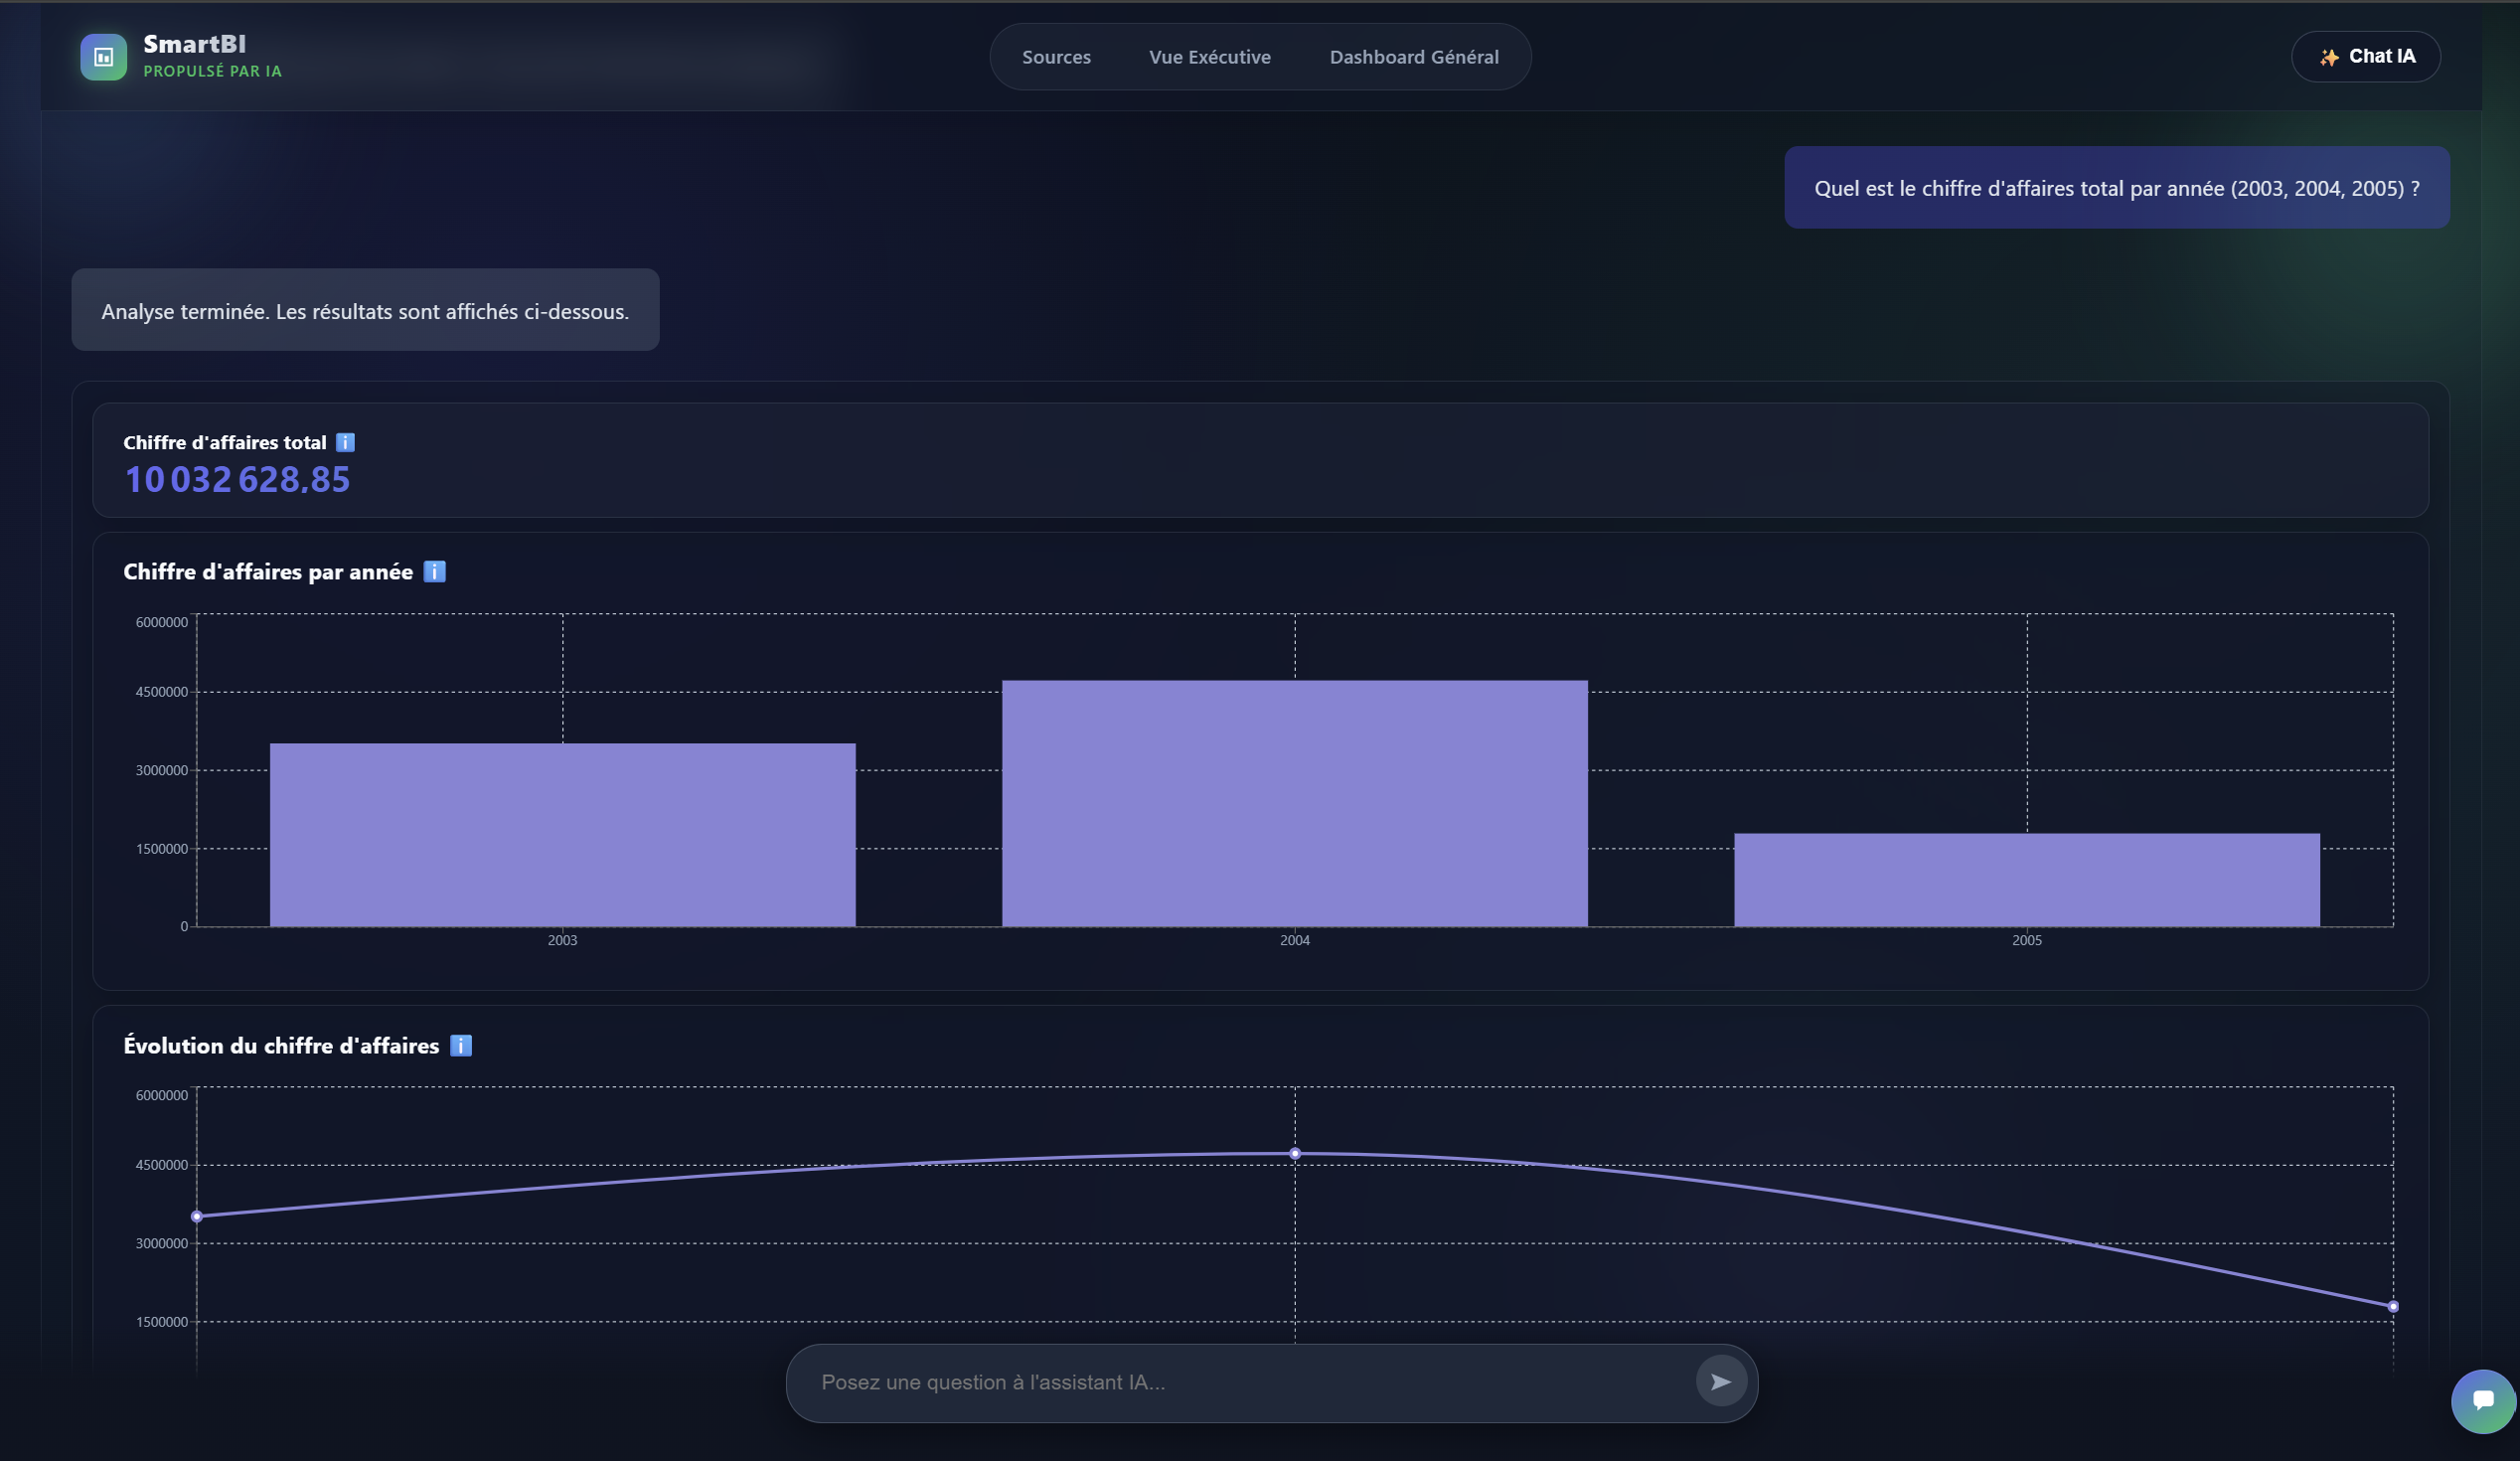
\includegraphics[width=\textwidth]{Smartbi/Screenshot 2026-06-22 181118.png}
\caption{Réponse conversationnelle avec graphique}
\label{fig:filtrage}
\end{figure}

\subsection{Scénario 3 : Auto-correction d'une erreur SQL}

Lors de la génération d'une requête, l'agent ingénieur peut produire une requête utilisant une syntaxe incompatible avec SQLite. L'exécution échoue et l'erreur est capturée. Au second essai, le prompt inclut le message d'erreur et l'agent corrige automatiquement sa requête. Ce mécanisme de retry avec feedback assure un taux de succès élevé pour la génération SQL.

\section{Difficultés rencontrées et solutions}

\subsection{Fiabilité de la génération SQL}

La génération de SQL par un LLM présente un taux d'erreur non négligeable, notamment pour les fonctions de date spécifiques à SQLite et les agrégations imbriquées. Le mécanisme de retry avec feedback d'erreur s'est révélé efficace : dans la majorité des cas, la deuxième tentative produit une requête correcte.

\subsection{Latence du pipeline}

L'exécution séquentielle des trois agents induit une latence cumulée de 30 à 60 secondes. Le streaming NDJSON pour l'upload atténue cette latence perçue en fournissant un retour visuel continu. Pour le mode conversationnel, un indicateur de chargement informe l'utilisateur.

\subsection{Qualité des visualisations}

La pertinence des visualisations dépend de la capacité du LLM à choisir le type de graphique approprié. Des instructions explicites dans les prompts du designer (PieChart pour les distributions, LineChart pour les séries temporelles, etc.) améliorent significativement les résultats.

\section{Synthèse}

La phase de réalisation a abouti à un prototype fonctionnel complet. SmartBI est capable de recevoir un fichier de données, de l'analyser automatiquement via un pipeline multi-agents, de générer des tableaux de bord interactifs et de répondre à des questions en langage naturel. Les mécanismes d'auto-correction, de streaming de progression et de persistance de l'état contribuent à une expérience utilisateur fluide et professionnelle.
